\section{PhoenixSim}

El nombre de PhoenixSim proviene de \textit{Photonic and Electronic Network Integration} ó 
integración fotónica y electrónica de redes. Esta herramienta permite modelar y 
analizar el rendimiento de sistemas multiprocesador que usan redes electrónicas, fotónicas
o híbridas. PhoenixSim captura las características físicas y las métricas de los diferentes 
dispositivos de interconexión nanofotónicos y elementos de red que no poseen un equivalente
 electrónico \cite{Chan2010}.
 
Está desarrollado sobre la herramienta OMNeT++ para simulación de eventos discretos
\cite{varga2005omnet++} sobre la cuál se montó una librería de dispositivos fotónicos
y electrónicos altamente parametrizable.

Para el desarrollo de redes de interconexión sobre PhoenixSim, se recomienda seguir
las siguientes etapas metodológicas \cite{Chan2011} mostradas en la Figura \ref{fig:phoenix_ovw}:

\begin{itemize}
\item Especificar los dispositvos con los que se construirá la red.
\item Seleccionar la aplicación o aplicaciones que se ejecutarán sobre la red.
\item Modelar la aquitectura de la red
\item Analizar el rendimiento a nivel de sistema.
\item Caracterizar la red a nivel físico.
\item Refinamiento iterativo de los pasos anteriores (parámetros y diseño).
\end{itemize} 

\begin{figure}[H]
\caption{Vista General PhoenixSim. Fuente \cite{Chan2011}}
\centering
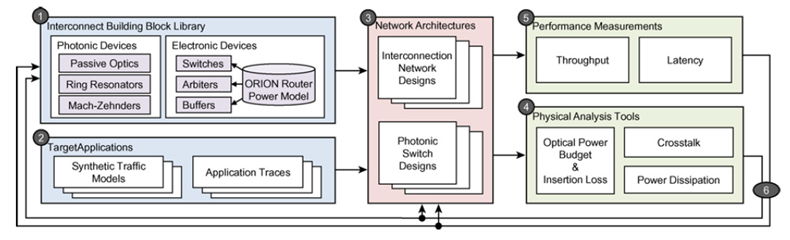
\includegraphics[width=1.0\textwidth,natwidth=790,natheight=240]{figs/overview.png}
\label{fig:phoenix_ovw}
\end{figure}

\subsection{Dispositivos de Interconexión}
\subsubsection{Electrónicos}

\paragraph{Router Electrónico}~\\
El router electrónico es usado tanto en las redes completamente electrónicas como en las fotónicas. En éstas últimas su uso se da a través del router híbrido, el cual lo necesita para controlar el camino por el cual serán enviados los datos en el plano fotónico.

\begin{itemize}
\item Puerto de Entrada (InPort)
\item Entramado de comunicación (Crossbar)
\item Controlador (Arbiter)
\end{itemize} 

\subsubsection{Fotónicos}
PhoenixSim abstrae las características físicas más importantes de los elementos fotónicos (capítulos \ref{ch:intro} y \ref{ch:rr}) sin perder la presición de sus resultados y sin necesidad de realizar una simulación FDTD completa. 

Al usar sólo las características más relevantes, se pueden emplear como componentes de las diferentes redes al mismo tiempo que se mantiene el rendimiento de la simulación a nivel de sistema.
Existen 2 categorías: activos y pasivos. La diferencia radica en que el comportamiento 
de los dispositivos pasivos o estáticos no cambia durante la ejecución de la simulación.

\paragraph{Pasivos}~\\
\begin{itemize}
\item Guía de onda

Representa el cable óptico con el que se conectan los demás dispositivos fotónicos. 
Presentan pérdidas por inserción debido a la atenuación que experimenta la onda
al viajar a través de la estructura. Otros factores influyen son 
las dimensiones de la guía, las propiedades de los materiales usados y las técnicas
de fabricación.

Este dispositivo está caracterizado por los 3 parámetros  mostrados en 
las tablas \ref{tb:wg_params} y \ref{tb:phpar_wg}.

\begin{table}[H]
\centering
\begin{tabular}{|c|c|c|}
\hline
Descripción &  Nombre Parámetro & Abv. \\
\hline
Longitud & $Length$ & $L_{wg}$ \\
Latencia & $LatencyRate\_Line$ & $t_{wg}$ \\
Pérdidas por Propagación & $PropagationLoss$ & $\alpha_{wg}$ \\
\hline
\end{tabular}
\caption{Caracterización Guía de Onda.}
\label{tb:wg_params}
\end{table} 

En PhoenixSim la guía de onda es modelada como un sistema con 2 puertos de entrada
y 2 puertos de salida. Como se ve en la figura \ref{fig:phoenix_wg}, este sistema
posee una tabla de enrutamiento $[1,0]$ donde el índice representa el puerto de entrada
y el valor indica el puerto por el que sale la señal. Es decir, la señal óptica que ingresa
por el puerto 0 sale por el puerto 1 y viceversa. \cite{Chan2011}

\begin{figure}[H]
\caption{Caracterización: Guía de Onda. Fuente: Autor.}
\centering
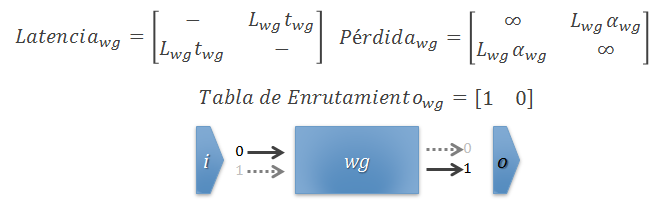
\includegraphics[width=0.9\textwidth,natwidth=665,natheight=200]{figs/wg.png}
\label{fig:phoenix_wg}
\end{figure}

Finalmente, para dar una idea de la implementación de este componente, se extrajo la siguiente
sección de código del archivo $line.cc$ de PhoenixSim.

\zcodectl{"sources/c2_wg.cpp"}{Implementación de la guía de onda en PhoenixSim.} 


\item Guía de onda doblada

Este tipo de estructura es requerido con el fin de cambiar la trayectoria de una señal en
un ángulo no mayor a 90 grados. Presentan pérdidas por inserción adicionales a las de 
la guía de onda recta (\textit{BendingLoss}) debido a 
los dobleces \cite{Chan2011}. Están modelados por los parámetros de la tabla \ref{tb:wgb_params} 
y \ref{tb:phpar_wgb}.

\begin{table}[H]
\centering
\begin{tabular}{|c|c|c|}
\hline
Descripción &  Nombre Parámetro \\
\hline
Ángulo & $Angle\_Bend$ \\
Latencia & $Latency\_Bend$ \\
Pérdidas por Propagación & $PropagationLoss$ \\
Pérdidas por doblez & $BendingLoss$ \\
\hline
\end{tabular}
\caption{Caracterización Guía de Onda.}
\label{tb:wgb_params}
\end{table} 


\item Cruce de guías de onda

Los cruces en una topología de red se presentan debido a la naturaleza planar o 2D 
de la plataforma tecnológica sobre la cual están construidas. Esta situación se da cada vez que 
2 guías de onda recta se intersectan presentando tanto pérdidas por inserción como diafonía 
(\textit{crosstalk}) \cite{Chan2010}. Este efecto es minimizado gracias a técnicas de fabricación donde 
se amplía y se emplea un doble borde en el área de cruce \cite{bogaerts2007low}.
Este fenómeno no se presenta en las interconexiones electrónicas ya que generaría un corto
circuito. 

Este dispositivo está modelado como un sistema de 4 entradas y 4 salidas como se ve en la 
figura \ref{fig:phoenix_wgc} y por los parámetros de la tabla \ref{tb:phpar_wgc}.
\begin{figure}[H]
\caption{Caracterización: Cruce de Guía de Onda. Fuente: Autor.}
\centering
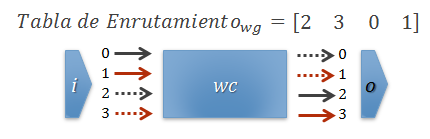
\includegraphics[width=0.6\textwidth,natwidth=430,natheight=139]{figs/wgcross.png}
\label{fig:phoenix_wgc}
\end{figure}

\item Acoplador

Un acoplador es una interfaz óptica entre los dominios dentro y fuera del chip. 
Es decir, es capaz de transferir una onda de un médio de propagación (como una
fibra óptica) hacia otro (como una guía de onda) y es prácticamente transparente
a la distancia de propagación \cite{Chan2011}.

Se modela como un dispositivo de 2 puertos con un sólo parámetro para demarcar
las pérdidas por inserción.

\end{itemize}

\paragraph{Activos}~\\

Estos dispositivos son unos de los elementos principales
empleados en Silicon Photonics y están basados los en anillos 
resonadores (Capítulo \ref{ch:rr}).

Como se vio en (\ref{eq:mode_l}) y (\ref{eq:mode_l+1}) las señales ópticas se acoplan
en el resonador a longitudes de onda específicas llamadas modos resonantes. 
Estos modos están separados periódicamente por el parámetro FSR (\ref{eq:fsr}) 
el cuál es inversamente proporcional al diámetro del anillo. Es decir, que anillos
con radio grande tienen un espaciamiento entre los modos pequeño y viceversa.
Como se analizó en la anterior fase, el FSR puede ser ajustado variando
el tamaño físico del radio, pero también mediante cambios en el índice de refracción
del anillo. Para esto, se pueden emplear 2 técnicas: mediante alteraciones térmicas,
o mediante la aplicación de un voltaje (Figura \ref{fig:phoenix_wgc}(a)) \cite{Chan2010}.

Debido a estas características, este elemento puede ser diseñado para realizar 
tareas de ruteo, modulación y recepción de señales ópticas. Es decir, puede ser
diseñado para comportarse como:

\begin{figure}[H]
\caption{(a). Cambio de estado de resonancia on-off
al aplicar un voltaje Fuente \cite{hendry2011time}. (b). Caracterización: Anillo Resonador. Fuente: Autor.}
\centering
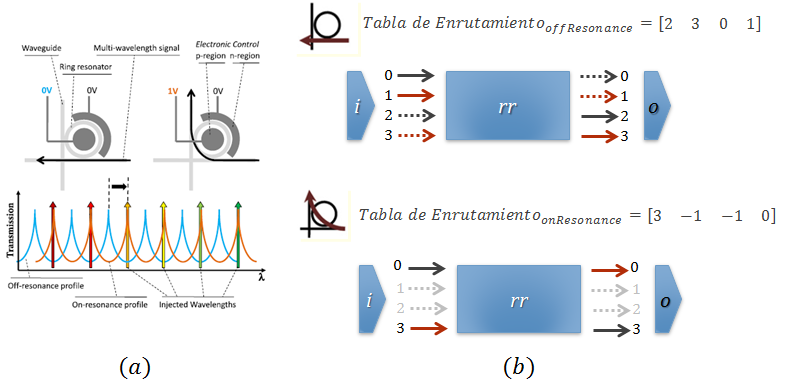
\includegraphics[width=1.0\textwidth,natwidth=800,natheight=390]{figs/rr.png}
\label{fig:phoenix_wgc}
\end{figure}

\begin{itemize}
\item Filtros:
Este dispositivo trabaja sobre una longitud específica y por eso es diseñado 
para tener una separación alta entre los modos (FSR alto), es decir que el 
tamaño del diámetro de estos dispositivos es pequeño. En \cite{little1998ultra} 
se demuestran filtros basados en anillos de $3\mu m$.

\item Switches de banda ancha
En este caso se requiere poder manipular o rutear un conjunto de longitudes
de onda al mismo tiempo. Es decir que se requiere un FSR pequeño donde, cuando
el anillo esté activo (estado ON), las frecuencias de interés estén alineadas con los
modos de resonancia del anillo y cuando esté apagado (OFF), se altere el índice
de refracción de tal forma que dejen de entrar en resonancia.
Debido al FSR pequeño requerido, estos anillos son de mayor tamaño que los filtros.

\item Moduladores
Estos dispositivos codifican un conjunto de datos electrónicos en
una longitud de onda específica. Esta selectividad requerida signfica
que el dispositivo tiene un FSR alto, es decir, se comporta similar
al filtro mencionado anteriormente.

\item Detectores
Los anillos resonadores aunque no se comportan como dispositivos de detección
propiamente, si son una pieza complementaria a estos, ya que realizan 
el filtrado de las longitudes de onda específicas antes de pasarlo
al dispositivo de detección.

\end{itemize}  


\subsection{Benchmarks}
\subsubsection{Modelos de Patrones Sintéticos}
\label{sss:synthetic}

\paragraph{Random}~\\
Ejecuta un tráfico aleatorio sobre la red. Cada core selecciona un core destino aleatoriamente
mediante una distribución uniforme. Una vez enviado, espera un tiempo dado por el parámetro
\textit{appParam1} para enviar un nuevo mensaje \cite{Manual}.

\paragraph{Neighboor}~\\
Realiza el envío de mensajes de cada core a sus vecinos \cite{hendry2009analysis}.

\paragraph{BitReverse}~\\
Patrón de envío de mensajes diseñado para realizar pruebas de estrés sobre topologías NoC 2D.
Cada core envía un mensaje a una dirección que corresponde a su dirección inversa a nivel de
bits. Este tipo de comunicación, los mensajes deben viajar trayectos largos que atraviezan la 
red \cite{hendry2009analysis}.

\paragraph{Tornado} ~\\
Otro patrón de envío de mensajes que realiza pruebas de estrés sobre Mesh 2D al hacer que
cada core se comunique con el vecino de su vecino. Es una versión competitiva del patrón
Neighboor \cite{hendry2009analysis}.

\begin{figure}[H]
\caption{Patrones sintéticos. Fuente \cite{hendry2009analysis}}
\centering
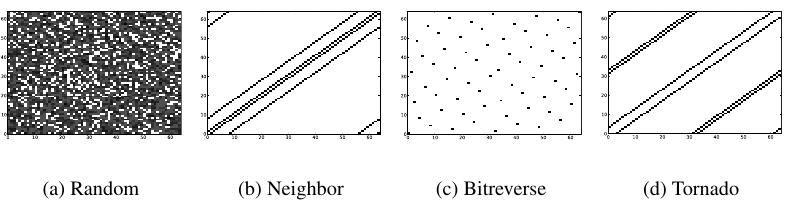
\includegraphics[width=1.0\textwidth,natwidth=787,natheight=205]{figs/syntbench.png}
\label{fig:synthbench}
\end{figure} 

\paragraph{All2All}~\\ 
Permite probar que todas las rutas de comunicación entre los nodos sean accesibles. Esto permite evaluar el peor caso de pérdida por inserción en la red fotónica \cite{Manual}.

\paragraph{Pruebas de Memoria DRAM}~\\
Las pruebas sobre la memoria están divididas en 3 según la característica que se desee analizar: 
\begin{itemize}
\item One2One comunica un procesador y un módulo de memoria DRAM. Esto premite probar la latencia de los accesos a memoria cuando no hay carga en la red (zero-load latency).
\item One2All comunica un procesador hacia todos los módulos de memoria DRAM, con lo que se puede determinar la accesibilidad de estos.
\item All2One prueba el mecanismo de contención al generar un patrón de comunicación de estrés donde todos los procesadores acceden a un solo módulo de memoria.
\end{itemize} 

\subsubsection{Modelos de Aplicaciones Reales}
\paragraph{Transformada rápida de Fourier (FFT)}~\\

Está dividido en las etapas del algoritmo de Cooley-Turkey. La etapa principal es la que toma el mayor tiempo, 
Los tiempos de cada etapa deben ser pasados como parámetros de la simulación. Los valores por defecto incluidos en el \textit{textbed} de PhoenixSim fueron obtenidos de la caracterización  dada por Frigo y Johnson \cite{benchFFT} usando 8 núcleos de procesamiento. 

\subsubsection{Tipos de Redes}

Existe 3 tipos diferentes de redes implementadas en PhoenixSim: electrónicas basadas en créditos,
fotónicas híbridas conmutadas o con arbitraje basado en longitud de onda como la empleada
en \cite{hendry2011time}.

A continuación se explica el tipo de red que será empleado en esta fase de la investigación:

\paragraph{Fotónicas Híbridas Conmutadas}~\\

El plano de comunicación entre los cores 
está compuesta por una subred de control electrónica y la subred de datos
fotónica -es por esto que recibe el nombre de red híbrida.
La subred electrónica se encarga de establecer
un camino entre el origen y el destino de la comunicación mediante
negociaciones entre los routers involucrados en el camino del mensaje.
Una vez se recibe un mensaje de confirmación de que el 
camino puede ser asignado, este plano de control se encarga también de 
generar las señales eléctricas que configuran los dispositivos fotónicos 
para que establezcan el camino por el cual viajarán los datos sobre la
red fotónica.

